\RequirePackage{luatex85}
\documentclass[tikz, border=10pt]{standalone}

\usepackage[compat=1.1.0]{tikz-feynman}

\begin{document}

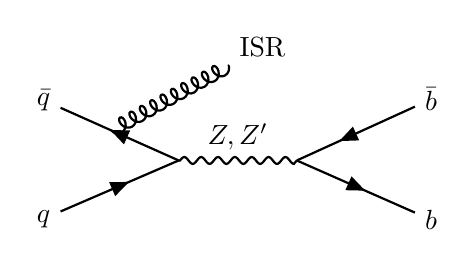
\begin{tikzpicture}[thick]
 \begin{feynman}
  \vertex (origin);
  \vertex [right=1.5cm of origin] (X);
  \vertex [above right=0.50cm and 1.5cm of X] (b1) {\(\bar{b}\)};
  \vertex [below right=0.50cm and 1.5cm of X] (b2) {\(b\)};
  \vertex [above left=0.50cm and 1.5cm of origin] (g1) {\(\bar{q}\)};
  \vertex [below left=0.50cm and 1.5cm of origin] (g2) {\(q\)};
  \vertex at ($(g1)!0.5!(origin)$) (ISR_start);
  \vertex [above right=0.8cm and 1.5 cm of ISR_start] (ISR) {ISR};
  \diagram* {
  (origin) -- [boson, edge label={\(Z,Z'\)}] (X) -- [anti fermion] (b1),
  (X) -- [fermion] (b2),
  (origin) -- [fermion] (g1),
  (g2) -- [fermion] (origin),
  (ISR_start) -- [gluon] (ISR),
  };
 \end{feynman}
\end{tikzpicture}
\end{document}
